\subsection{Surface Backgrounds}
% @Fei
Just add the content to start, will modify the description further.....

Interactions in the inner part of the detector can be nicely modelled by combining our knowledge on LXe's properties to ionizing particles and the detector related properties like charge/light collections. In cases where the latter information is missing/incomplete, we need to develop new algorithms to model the events. In this and following sections, two classes of background components are analyzed for the XENON1T dark matter searches.

As has been proved by several experiments~\cite{cdms, deap}, detector surfaces exposed long to ambient air during construction phase are contaminated by large amount of radon progeny, in particular the $^{210}$Pb. With a 22\,y half-life, $^{210}$Pb basically decays constantly within the XENON1T's operation of a few years. For dark matter searches, ion recoil of $^{206}$Pb from $^{210}$Po $\alpha$-decays, $\beta$-decays and the resulting X-rays, Auger electrons of $^{210}$Pb are particularly important. Due to unknown LXe's properties and detector physics in presence of PTFE as well as the complicated decay structures, a precise modeling based on Monte-Carlo simulation approach has not been achieved in XENON1T yet. Instead, a data driven approach is adopted to predict the event distribution of this background. 




\begin{figure}[tbp]
\centering
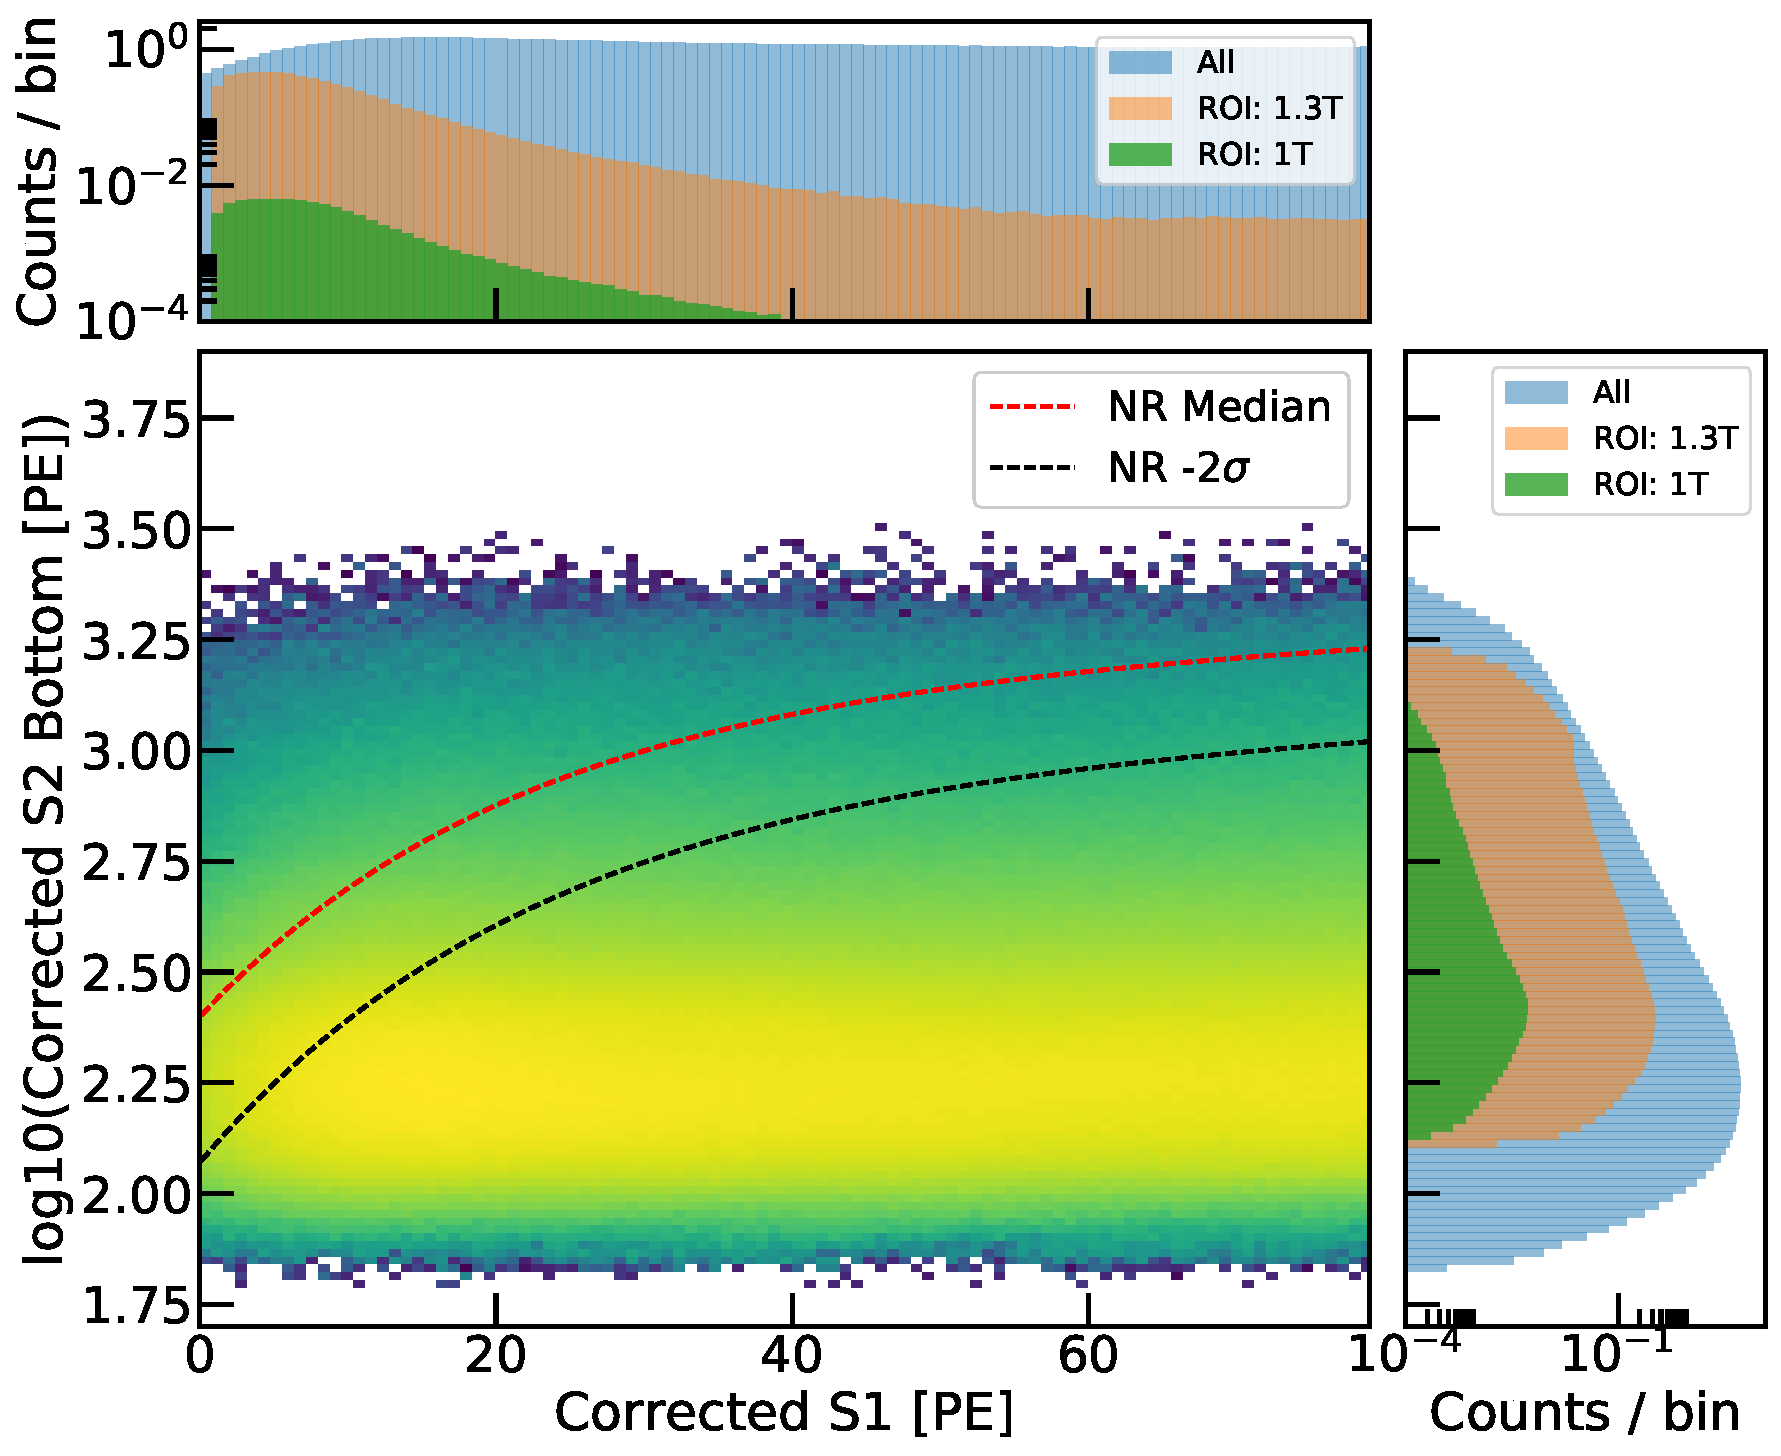
\includegraphics[width=\columnwidth]{Plots/surface_s2s1_distribution_blessed_sr1.pdf}
\caption{\label{fig:surface_bg} 
}
\end{figure}



